\chapter{Optimum Assignment Example}

\begin{proof}
    The next picture represents the adjacency matrix of a bipartite graph.
    The entries are the weight of each edge. The non-positive entries
    are colored in gray because in an optimum assignment problem they
    should be ignored.
    
    \begin{center}
        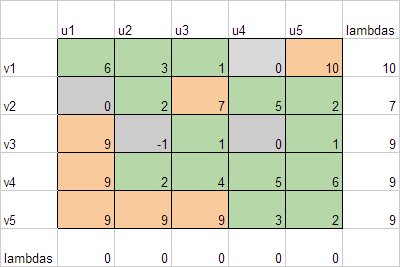
\includegraphics[width=10cm]{Homework2/OptimumAssignment1.png}    
    \end{center}\pn
    
    In the firs step, we assign the values of the dual variable \textit{lambda} 
    to be the maximum number of each row for the ``row vertices'' and zero
    for the ``column vertices''. (The name ``dual variable'' is given
    because of \href{http://www.mpi-inf.mpg.de/departments/d1/teaching/ss12/AdvancedGraphAlgorithms/Slides06.pdf}{these slides}).\pn
    
    Then we color red a (not necessarily perfect) matching of maximum weight.\pn 
    
    \begin{center}
        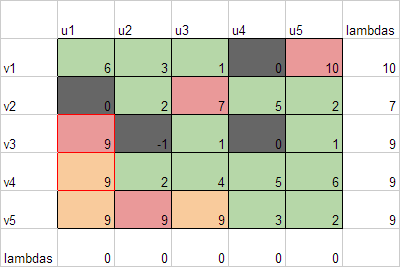
\includegraphics[width=10cm]{Homework2/OptimumAssignment2.png}        
    \end{center}\pn
    
    In the next steps we are going to try to construct an aumenting path on
    a tree rooted in a not covered vertex ($v_4$ in this example) by using
    the Hungarian algorithm.\pn
    
    Cells in orange are cells representing edges such that its weight is equal to the
    sum of the dual variable evaluated in its adjacent vertices and that
    not belong to the matching.\pn
    
    Cells with red border represent the edges in the tree.\pn
    
    In the next step, we modify the dual variable \textit{lambda} by substracting
    $3$ to its values on ``row vertices'' that belong to the tree and by adding
    $3$ to its values on ``column vertices'' that belong to the tree.\pn
    
    $3$ is the minimum weight needed to add new orange cells that could extend
    our tree.\pn
   
    \begin{center}
        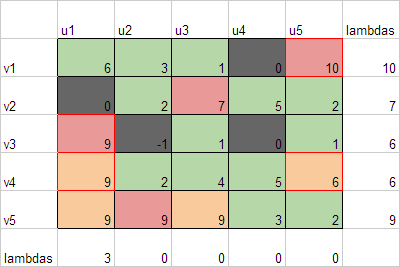
\includegraphics[width=10cm]{Homework2/OptimumAssignment3.png}
    \end{center}\pn

    After the addition of the new orange cells we extend the tree looking for an
    augmenting path. If we can't find one, then we repeat the steps from the one
    in which we modify the dual variable \textit{lambda}. 
    
    The next picture shows this repeating steps but now buy substracting and adding $1$
    instead of $3$.

    \begin{center}
        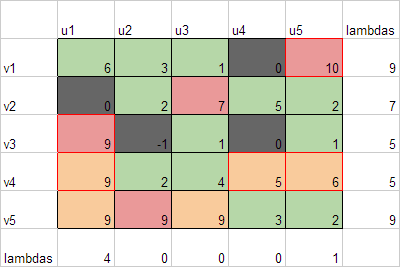
\includegraphics[width=10cm]{Homework2/OptimumAssignment4.png}
    \end{center}\pn

    Finally, the only edge added in this last step starts and ends in uncovered
    vertices. So this edge by itself is an augmenting path wich can complete
    an optimum assignment by being added to the matching.\pn
    
    In the next picture we show the optimum matching.\pn

    \begin{center}
        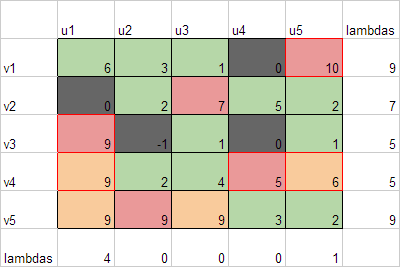
\includegraphics[width=10cm]{Homework2/OptimumAssignment5.png}
    \end{center}
\end{proof}